\chapter{向量代数}

% SOURCE_PDF_PAGE 219

\hypertarget{source-p219}{}
\phantomsection\addcontentsline{toc}{section}{4.1 竞赛要点与难点}
\phantomsection\addcontentsline{toc}{section}{4.2 范例解析与精讲}
从数学的观点研究向量的特性以及它的各种运算.向量方法不仅能使某些几何问题
得到简洁的解决，而且也是力学、物理学和工程技术中常用的有力工具.在建立了空间坐
标系后，向量与它的坐标间有了一一对应关系.这样就使得许多涉及向量之间的几何问题
转化成坐标之间的代数问题，为应用代数方法解决几何问题提供了桥梁.
\section*{4.1 竞赛要点与难点}
\par\noindent (1) 向量的定义、表示、向量的线性运算、向量的分解、几何运算.
\par\noindent (2) 坐标系的概念、向量与点的坐标及向量的代数运算.
\par\noindent (3) 向量在轴上的射影及其性质、方向余弦、向量的夹角.
\par\noindent (4) 向量的数量积、向量积、混合积以及二重外积的定义、几何意义、运算性质、计
算方法及应用.
\par\noindent (5) 应用向量求解一些几何、三角问题.
\section*{4.2 范例解析与精讲}
\sourceblock{450.00}{images-full/p219-type1.png}
用\allowbreak{}\raisebox{-2.64pt}{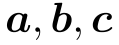
\includegraphics[width=33.33pt]{images-full/p219-i000.png}}\allowbreak{} 表示几何空间的向量，用\allowbreak{}\raisebox{-3.60pt}{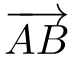
\includegraphics[width=20.90pt]{images-full/p219-i001.png}}\allowbreak{} 表示]\allowbreak{}\raisebox{-2.76pt}{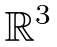
\includegraphics[width=15.82pt]{images-full/p219-i002.png}}\allowbreak{} 中始点为$A$，终点为$B$ 的向量.
\par\noindent (1) 向量\allowbreak{}\raisebox{-1.68pt}{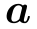
\includegraphics[width=10.17pt]{images-full/p219-i005.png}}\allowbreak{} 与向量$b$ 的内积定义为
\sourceblock{127.12}{images-full/p219-d000.png}
\sourceblock{393.80}{images-full/p219-d001.png}
\par\noindent (2) 向量\allowbreak{}\raisebox{-1.68pt}{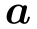
\includegraphics[width=10.17pt]{images-full/p219-i007.png}}\allowbreak{} 与$b$ 的外积\allowbreak{}\raisebox{-2.28pt}{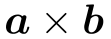
\includegraphics[width=31.07pt]{images-full/p219-i009.png}}\allowbreak{} 仍然是一个向量，同时正交于\allowbreak{}\raisebox{-1.68pt}{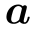
\includegraphics[width=10.17pt]{images-full/p219-i010.png}}\allowbreak{} 与$b$，其长度为
\sourceblock{235.60}{images-full/p219-d002.png}
几何空间上表示以\allowbreak{}\raisebox{-1.68pt}{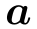
\includegraphics[width=10.17pt]{images-full/p219-i012.png}}\allowbreak{} 和$b$ 张成的平行四边形的面积.
\par\noindent (3) 向量\allowbreak{}\raisebox{-2.76pt}{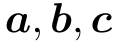
\includegraphics[width=33.33pt]{images-full/p219-i014.png}}\allowbreak{} 的混合积
\sourceblock{194.36}{images-full/p219-d003.png}


% SOURCE_PDF_PAGE 220

\hypertarget{source-p220}{}
其中\allowbreak{}\raisebox{-2.88pt}{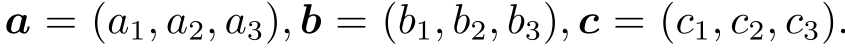
\includegraphics[width=238.42pt]{images-full/p220-i000.png}}\allowbreak{} 温合积的绝对植等于由\allowbreak{}\raisebox{-2.76pt}{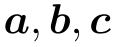
\includegraphics[width=33.33pt]{images-full/p220-i001.png}}\allowbreak{} 所张
成的平行六面体的体积.
需要指出的是，当不致引起混淆时，本书也用记号\allowbreak{}\raisebox{-3.00pt}{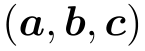
\includegraphics[width=40.68pt]{images-full/p220-i002.png}}\allowbreak{} 表示由向量\allowbreak{}\raisebox{-2.76pt}{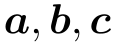
\includegraphics[width=33.33pt]{images-full/p220-i003.png}}\allowbreak{} 构成的
列分块矩阵
\par\noindent (4) 设\allowbreak{}\raisebox{-3.12pt}{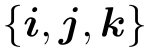
\includegraphics[width=42.37pt]{images-full/p220-i004.png}}\allowbreak{} 为几何空间\allowbreak{}\raisebox{-2.64pt}{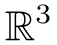
\includegraphics[width=15.82pt]{images-full/p220-i005.png}}\allowbreak{}的直角坐标系，其中\allowbreak{}\raisebox{-2.88pt}{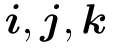
\includegraphics[width=31.64pt]{images-full/p220-i006.png}}\allowbreak{} 是彼此正交的单位向量，
则对于任意的\allowbreak{}\raisebox{-3.12pt}{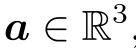
\includegraphics[width=38.13pt]{images-full/p220-i007.png}}\allowbreak{}，有\allowbreak{}\raisebox{-2.76pt}{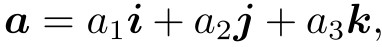
\includegraphics[width=107.64pt]{images-full/p220-i008.png}}\allowbreak{}，筒记为\allowbreak{}\raisebox{-3.00pt}{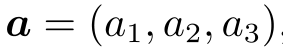
\includegraphics[width=79.84pt]{images-full/p220-i009.png}}\allowbreak{}，称为向量\allowbreak{}\raisebox{-1.68pt}{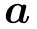
\includegraphics[width=10.17pt]{images-full/p220-i010.png}}\allowbreak{} 的坐
标表示.向量组\allowbreak{}\raisebox{-2.76pt}{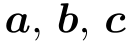
\includegraphics[width=37.29pt]{images-full/p220-i011.png}}\allowbreak{} 线性无关的充要条件是满足
\sourceblock{283.06}{images-full/p220-d000.png}
的\allowbreak{}\raisebox{-2.16pt}{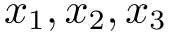
\includegraphics[width=48.02pt]{images-full/p220-i012.png}}\allowbreak{} 均为零.若满足(4.2.1) 的\allowbreak{}\raisebox{-2.16pt}{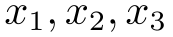
\includegraphics[width=48.59pt]{images-full/p220-i013.png}}\allowbreak{}不全为零，则称\allowbreak{}\raisebox{-2.76pt}{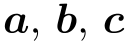
\includegraphics[width=37.29pt]{images-full/p220-i014.png}}\allowbreak{}线性相关.
\par\noindent (5) 向量运算的性质.
设\allowbreak{}\raisebox{-3.00pt}{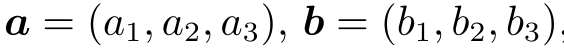
\includegraphics[width=159.23pt]{images-full/p220-i015.png}}\allowbreak{})，则有
\par (5.1) 向量加法:\allowbreak{}\raisebox{-2.88pt}{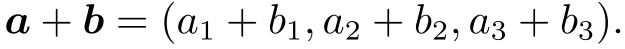
\includegraphics[width=176.23pt]{images-full/p220-i016.png}}\allowbreak{}
\par (5.2) 向量减法:\allowbreak{}\raisebox{-3.00pt}{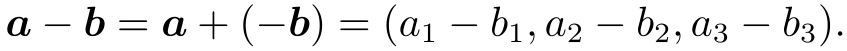
\includegraphics[width=239.09pt]{images-full/p220-i017.png}}\allowbreak{}
\par (5.3) 数乘向量:\allowbreak{}\raisebox{-3.00pt}{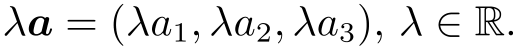
\includegraphics[width=144.59pt]{images-full/p220-i018.png}}\allowbreak{}
\sourceblock{389.85}{images-full/p220-d001.png}
\par (5.9) 设\allowbreak{}\raisebox{-3.00pt}{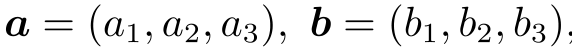
\includegraphics[width=161.46pt]{images-full/p220-i019.png}}\allowbreak{}，则
\sourceblock{210.18}{images-full/p220-d002.png}
\sourceblock{235.04}{images-full/p220-d003.png}
\par\medskip\noindent\textbf{【例4.2.1 】设a ，b，c ε 1R.a线性无关，对任意hε 肘，求h 关于\allowbreak{}\raisebox{-2.64pt}{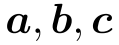
\includegraphics[width=33.33pt]{images-full/p220-i020.png}}\allowbreak{} 的线性表}
示式.
解因为\allowbreak{}\raisebox{-2.76pt}{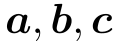
\includegraphics[width=33.33pt]{images-full/p220-i021.png}}\allowbreak{} 线性无关，所以$h$ 可由\allowbreak{}\raisebox{-2.76pt}{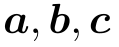
\includegraphics[width=33.33pt]{images-full/p220-i023.png}}\allowbreak{} 线性表示，设为
\sourceblock{113.56}{images-full/p220-d004.png}
用\allowbreak{}\raisebox{-2.28pt}{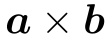
\includegraphics[width=31.07pt]{images-full/p220-i024.png}}\allowbreak{} 对上式两边作内积，得
\sourceblock{297.19}{images-full/p220-d005.png}
注意到
\sourceblock{148.59}{images-full/p220-d006.png}


% SOURCE_PDF_PAGE 221

\hypertarget{source-p221}{}
所以
\sourceblock{206.22}{images-full/p221-d000.png}
困为\allowbreak{}\raisebox{-2.76pt}{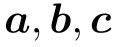
\includegraphics[width=33.33pt]{images-full/p221-i000.png}}\allowbreak{} 线性无关，所以忡\allowbreak{}\raisebox{-3.00pt}{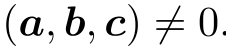
\includegraphics[width=63.64pt]{images-full/p221-i001.png}}\allowbreak{} 故由上式可得
\sourceblock{77.40}{images-full/p221-d001.png}
类似地，可得
\sourceblock{164.41}{images-full/p221-d002.png}
因此，$h$ 关于\allowbreak{}\raisebox{-2.76pt}{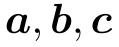
\includegraphics[width=33.33pt]{images-full/p221-i003.png}}\allowbreak{} 的线性表示式为
\sourceblock{208.48}{images-full/p221-d003.png}
\sourceblock{278.54}{images-full/p221-d004.png}
\sourceblock{436.74}{images-full/p221-d005.png}
其中\allowbreak{}\raisebox{-3.12pt}{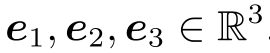
\includegraphics[width=75.96pt]{images-full/p221-i004.png}}\allowbreak{}. 证明:
\sourceblock{220.91}{images-full/p221-d006.png}
\par\noindent\textbf{证明}\ 因为
\sourceblock{376.85}{images-full/p221-d007.png}


% SOURCE_PDF_PAGE 222

\hypertarget{source-p222}{}
所以
\sourceblock{324.87}{images-full/p222-d000.png}
其中(\allowbreak{}\raisebox{-3.00pt}{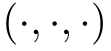
\includegraphics[width=31.07pt]{images-full/p222-i000.png}}\allowbreak{})表示由向量\allowbreak{}\raisebox{-2.64pt}{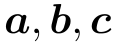
\includegraphics[width=33.33pt]{images-full/p222-i001.png}}\allowbreak{} 构成的矩阵对(4.2.2) 两端取行列式可得
\sourceblock{423.75}{images-full/p222-d001.png}
\par\medskip\noindent\textbf{【例4.2.4 】证明:设A ，B 是不同的两点，则点$M$ 在线段AB 上的充分必要条件}
\sourceblock{402.28}{images-full/p222-d002.png}
\sourceblock{307.36}{images-full/p222-d003.png}
\par\noindent\textbf{证明}\ 必要性设点$M$ 在线段\allowbreak{}\raisebox{-2.28pt}{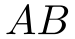
\includegraphics[width=20.90pt]{images-full/p222-i004.png}}\allowbreak{} 上，则存在\allowbreak{}\raisebox{-2.88pt}{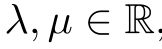
\includegraphics[width=45.42pt]{images-full/p222-i005.png}}\allowbreak{}R，且\allowbreak{}\raisebox{-2.88pt}{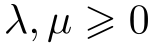
\includegraphics[width=44.03pt]{images-full/p222-i006.png}}\allowbreak{} (不同时为零)，
使得
\sourceblock{92.66}{images-full/p222-d004.png}
\sourceblock{391.54}{images-full/p222-d005.png}
充分性设存在\allowbreak{}\raisebox{-2.76pt}{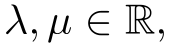
\includegraphics[width=48.02pt]{images-full/p222-i007.png}}\allowbreak{}，且\allowbreak{}\raisebox{-2.76pt}{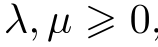
\includegraphics[width=44.25pt]{images-full/p222-i008.png}}\allowbreak{}，使得对空间中的任意一点\allowbreak{}\raisebox{-2.76pt}{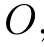
\includegraphics[width=12.12pt]{images-full/p222-i009.png}}\allowbreak{}，都有(4.2功式
成立，则
\sourceblock{326.00}{images-full/p222-d006.png}
因此点$M$ 在线段\allowbreak{}\raisebox{-2.40pt}{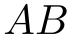
\includegraphics[width=20.90pt]{images-full/p222-i011.png}}\allowbreak{} 上.口
【注4.2.1 】本题结论在利用向量方法求解几何问题特别是有关线段的定比分点时
是很有用的工具.


% SOURCE_PDF_PAGE 223

\hypertarget{source-p223}{}
园也型二时附合刷品哇，卡在
\par\medskip\noindent\textbf{【例4.2.5 】证明二重外积公式}
\sourceblock{312.44}{images-full/p223-d000.png}
\par\noindent\textbf{证明}\ 令\allowbreak{}\raisebox{-3.00pt}{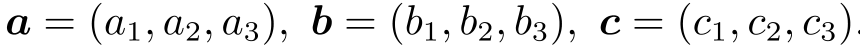
\includegraphics[width=242.79pt]{images-full/p223-i000.png}}\allowbreak{} 因为
\sourceblock{450.00}{images-full/p223-d001.png}
\par\medskip\noindent\textbf{【例4.2.6 】证明Jacobi (雅可比)恒等式}
\sourceblock{230.52}{images-full/p223-d002.png}
\par\noindent\textbf{证明}\ 利用二重外积公式(4.2.4)，得
\sourceblock{168.37}{images-full/p223-d003.png}
将上述三个式子相加即得所证等式.口
\par\medskip\noindent\textbf{【例4.2.7 】证明Lagrange 恒等式:对几何空间\allowbreak{}\raisebox{-2.76pt}{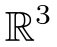
\includegraphics[width=15.82pt]{images-full/p223-i001.png}}\allowbreak{}中的任意向量\allowbreak{}\raisebox{-2.64pt}{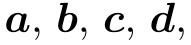
\includegraphics[width=53.46pt]{images-full/p223-i002.png}}\allowbreak{}恒有}
\sourceblock{170.06}{images-full/p223-d004.png}
\par\noindent\textbf{证明}\ 将\allowbreak{}\raisebox{-2.28pt}{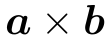
\includegraphics[width=31.07pt]{images-full/p223-i003.png}}\allowbreak{} 看作一个向量，根据混合积的性质并利用二重外积公式得
\sourceblock{184.19}{images-full/p223-d005.png}


% SOURCE_PDF_PAGE 224

\hypertarget{source-p224}{}
\sourceblock{262.72}{images-full/p224-d000.png}
\par\medskip\noindent\textbf{【例4.2.8 】证明:向量\allowbreak{}\raisebox{-2.76pt}{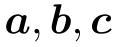
\includegraphics[width=33.33pt]{images-full/p224-i000.png}}\allowbreak{} 共面的充分必要条件是\allowbreak{}\raisebox{-2.76pt}{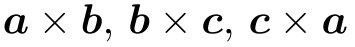
\includegraphics[width=100.00pt]{images-full/p224-i001.png}}\allowbreak{} 共面.}
\par\noindent\textbf{证明}\ (方法1) 问题可等价地证明:向量组\allowbreak{}\raisebox{-2.64pt}{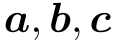
\includegraphics[width=33.33pt]{images-full/p224-i002.png}}\allowbreak{} 线性无关的充分必要条件是\allowbreak{}\raisebox{-2.64pt}{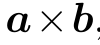
\includegraphics[width=27.84pt]{images-full/p224-i003.png}}\allowbreak{}，
\allowbreak{}\raisebox{-2.76pt}{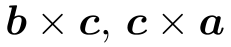
\includegraphics[width=64.97pt]{images-full/p224-i004.png}}\allowbreak{} 线性无关.事实上，若\allowbreak{}\raisebox{-2.76pt}{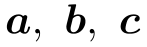
\includegraphics[width=41.24pt]{images-full/p224-i005.png}}\allowbreak{}线性无关，设
\sourceblock{201.14}{images-full/p224-d001.png}
用\allowbreak{}\raisebox{-1.68pt}{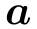
\includegraphics[width=10.17pt]{images-full/p224-i006.png}}\allowbreak{} 对上式两端作内积可得\allowbreak{}\raisebox{-3.00pt}{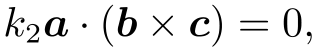
\includegraphics[width=88.16pt]{images-full/p224-i007.png}}\allowbreak{}，因为\allowbreak{}\raisebox{-3.00pt}{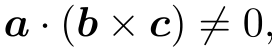
\includegraphics[width=76.46pt]{images-full/p224-i008.png}}\allowbreak{}，得到\allowbreak{}\raisebox{-2.64pt}{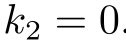
\includegraphics[width=35.27pt]{images-full/p224-i009.png}}\allowbreak{} 类似地
可得\allowbreak{}\raisebox{-2.64pt}{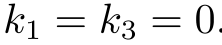
\includegraphics[width=62.62pt]{images-full/p224-i010.png}}\allowbreak{} 从而\allowbreak{}\raisebox{-2.76pt}{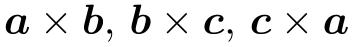
\includegraphics[width=100.00pt]{images-full/p224-i011.png}}\allowbreak{} 线性无关.
另一方面，若\allowbreak{}\raisebox{-2.64pt}{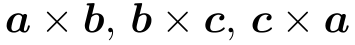
\includegraphics[width=100.00pt]{images-full/p224-i012.png}}\allowbreak{}线性无关，设
\sourceblock{108.48}{images-full/p224-d002.png}
用\allowbreak{}\raisebox{-1.68pt}{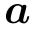
\includegraphics[width=10.17pt]{images-full/p224-i013.png}}\allowbreak{} 对上式两端作外积，可得
\sourceblock{138.42}{images-full/p224-d003.png}
因为\allowbreak{}\raisebox{-2.64pt}{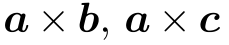
\includegraphics[width=64.41pt]{images-full/p224-i014.png}}\allowbreak{}线性无关，所以\allowbreak{}\raisebox{-2.64pt}{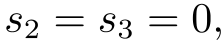
\includegraphics[width=62.49pt]{images-full/p224-i015.png}}\allowbreak{}，从而有\allowbreak{}\raisebox{-2.64pt}{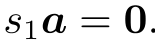
\includegraphics[width=43.39pt]{images-full/p224-i016.png}}\allowbreak{} 由于\allowbreak{}\raisebox{-2.88pt}{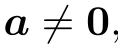
\includegraphics[width=33.24pt]{images-full/p224-i017.png}}\allowbreak{}，所以\allowbreak{}\raisebox{-2.64pt}{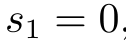
\includegraphics[width=35.23pt]{images-full/p224-i018.png}}\allowbreak{},
因此\allowbreak{}\raisebox{-2.76pt}{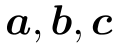
\includegraphics[width=33.33pt]{images-full/p224-i019.png}}\allowbreak{} 线性无关.
(方法2) 建立混合积\allowbreak{}\raisebox{-3.00pt}{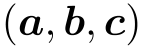
\includegraphics[width=40.68pt]{images-full/p224-i020.png}}\allowbreak{} 与\allowbreak{}\raisebox{-3.00pt}{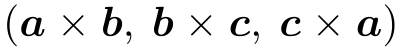
\includegraphics[width=113.00pt]{images-full/p224-i021.png}}\allowbreak{} 之间的关系式.事实上，将
\allowbreak{}\raisebox{-2.28pt}{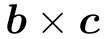
\includegraphics[width=29.94pt]{images-full/p224-i022.png}}\allowbreak{}看作一个向量，利用二重外积公式得
\sourceblock{254.81}{images-full/p224-d004.png}
所以
\sourceblock{263.29}{images-full/p224-d005.png}
因此，\allowbreak{}\raisebox{-2.88pt}{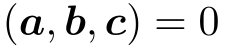
\includegraphics[width=63.28pt]{images-full/p224-i023.png}}\allowbreak{}等价于\allowbreak{}\raisebox{-3.00pt}{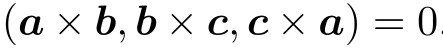
\includegraphics[width=124.79pt]{images-full/p224-i024.png}}\allowbreak{}. 这就证明了，向量\allowbreak{}\raisebox{-2.64pt}{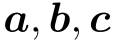
\includegraphics[width=33.33pt]{images-full/p224-i025.png}}\allowbreak{}共面的充分
必要条件是\allowbreak{}\raisebox{-2.76pt}{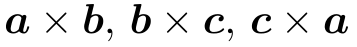
\includegraphics[width=100.57pt]{images-full/p224-i026.png}}\allowbreak{} 共面.口


% SOURCE_PDF_PAGE 225

\hypertarget{source-p225}{}
\par\medskip\noindent\textbf{【例4.2.9 】证明:对于几何空间\allowbreak{}\raisebox{-2.64pt}{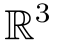
\includegraphics[width=15.82pt]{images-full/p225-i000.png}}\allowbreak{}中的任意向量\allowbreak{}\raisebox{-2.76pt}{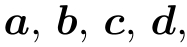
\includegraphics[width=52.67pt]{images-full/p225-i001.png}}\allowbreak{}恒有}
\sourceblock{257.64}{images-full/p225-d000.png}
\par\noindent\textbf{证明}\ (方法1) 依次将\allowbreak{}\raisebox{-2.28pt}{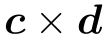
\includegraphics[width=30.51pt]{images-full/p225-i002.png}}\allowbreak{}与\allowbreak{}\raisebox{-2.28pt}{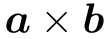
\includegraphics[width=31.07pt]{images-full/p225-i003.png}}\allowbreak{} 看作一个向量，利用二重外积公式得
\sourceblock{267.81}{images-full/p225-d001.png}
上述二式相减，即得所证等式.
(方法2) 设\allowbreak{}\raisebox{-2.64pt}{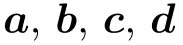
\includegraphics[width=51.41pt]{images-full/p225-i004.png}}\allowbreak{} 的直角坐标分别为
\sourceblock{359.34}{images-full/p225-d002.png}
\sourceblock{376.29}{images-full/p225-d003.png}
因为
\sourceblock{382.50}{images-full/p225-d004.png}
同理，得
\sourceblock{299.45}{images-full/p225-d005.png}
所以
\sourceblock{257.64}{images-full/p225-d006.png}


% SOURCE_PDF_PAGE 226

\hypertarget{source-p226}{}
(方法3) 若向量\allowbreak{}\raisebox{-2.76pt}{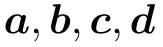
\includegraphics[width=45.76pt]{images-full/p226-i000.png}}\allowbreak{} 中的任意3 个的混合积都等于\allowbreak{}\raisebox{-2.64pt}{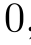
\includegraphics[width=8.34pt]{images-full/p226-i001.png}}\allowbreak{}，则等式显然成立.下面
考虑\allowbreak{}\raisebox{-2.16pt}{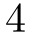
\includegraphics[width=8.47pt]{images-full/p226-i002.png}}\allowbreak{} 个混合积至少有一个不等于零，不妨设\allowbreak{}\raisebox{-3.00pt}{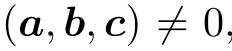
\includegraphics[width=65.02pt]{images-full/p226-i003.png}}\allowbreak{}，此时\allowbreak{}\raisebox{-2.76pt}{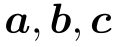
\includegraphics[width=33.33pt]{images-full/p226-i004.png}}\allowbreak{} 线性无关，因此
向量$d$ 可由\allowbreak{}\raisebox{-2.76pt}{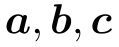
\includegraphics[width=33.33pt]{images-full/p226-i006.png}}\allowbreak{} 线性表示，设\allowbreak{}\raisebox{-2.76pt}{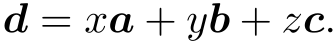
\includegraphics[width=93.92pt]{images-full/p226-i007.png}}\allowbreak{} 利用向量混合积的性质，得
\sourceblock{335.61}{images-full/p226-d000.png}
同理可得\allowbreak{}\raisebox{-2.88pt}{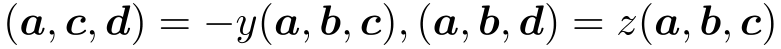
\includegraphics[width=220.35pt]{images-full/p226-i008.png}}\allowbreak{}，从而有
\sourceblock{450.00}{images-full/p226-d001.png}
团组型五旬机几何是周
利用向量方法解决几何问题，通常先将几何问题转化为向量的代数式(由向量及其运
算表示的式子)，再根据向量的各种运算与性质对代数式进行变形与简化，化归为具有明
显几何意义的代数式，从而使问题得到解决.
\sourceblock{450.00}{images-full/p226-d002.png}
\sourceblock{280.24}{images-full/p226-d003.png}
注意到\allowbreak{}\raisebox{-2.64pt}{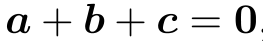
\includegraphics[width=74.06pt]{images-full/p226-i009.png}}\allowbreak{}，由此可得\allowbreak{}\raisebox{-3.48pt}{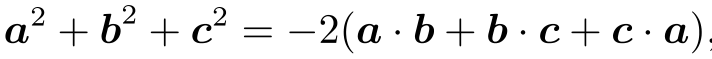
\includegraphics[width=200.91pt]{images-full/p226-i010.png}}\allowbreak{}，因此
\sourceblock{321.48}{images-full/p226-d004.png}
\sourceblock{129.38}{images-full/p226-d005.png}
图4.2.1


% SOURCE_PDF_PAGE 227

\hypertarget{source-p227}{}
\sourceblock{132.77}{images-full/p227-d000.png}
\sourceblock{450.00}{images-full/p227-d001.png}
\sourceblock{397.19}{images-full/p227-d002.png}
\sourceblock{401.15}{images-full/p227-d003.png}
\par\noindent (1) 证明:\allowbreak{}\raisebox{-2.40pt}{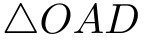
\includegraphics[width=40.91pt]{images-full/p227-i000.png}}\allowbreak{} 的面积为
\sourceblock{383.63}{images-full/p227-d004.png}
\sourceblock{197.75}{images-full/p227-d005.png}
比较上述两式，得
\sourceblock{83.05}{images-full/p227-d006.png}
\sourceblock{275.72}{images-full/p227-d007.png}
\sourceblock{77.97}{images-full/p227-d008.png}
困此\allowbreak{}\raisebox{-2.28pt}{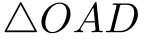
\includegraphics[width=41.24pt]{images-full/p227-i001.png}}\allowbreak{} 的面积为
\sourceblock{333.91}{images-full/p227-d009.png}


% SOURCE_PDF_PAGE 228

\hypertarget{source-p228}{}
\phantomsection\addcontentsline{toc}{section}{4.3 真题选讲与点评}
\sourceblock{341.82}{images-full/p228-d000.png}
\sourceblock{210.18}{images-full/p228-d001.png}
\sourceblock{450.00}{images-full/p228-d002.png}
易知，点\allowbreak{}\raisebox{-2.88pt}{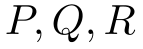
\includegraphics[width=40.11pt]{images-full/p228-i000.png}}\allowbreak{} 的仿射坐标为
\sourceblock{244.08}{images-full/p228-d003.png}
设\allowbreak{}\raisebox{-2.88pt}{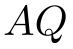
\includegraphics[width=20.34pt]{images-full/p228-i001.png}}\allowbreak{} 与\allowbreak{}\raisebox{-2.28pt}{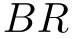
\includegraphics[width=21.47pt]{images-full/p228-i002.png}}\allowbreak{} 相交于点\allowbreak{}\raisebox{-2.88pt}{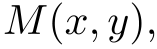
\includegraphics[width=44.11pt]{images-full/p228-i003.png}}\allowbreak{}且点$M$ 分别分线段\allowbreak{}\raisebox{-2.88pt}{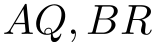
\includegraphics[width=44.63pt]{images-full/p228-i005.png}}\allowbreak{} 成定比\allowbreak{}\raisebox{-2.16pt}{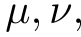
\includegraphics[width=22.75pt]{images-full/p228-i006.png}}\allowbreak{}，则
\sourceblock{361.60}{images-full/p228-d004.png}
\sourceblock{200.57}{images-full/p228-d005.png}
因此，\allowbreak{}\raisebox{-2.88pt}{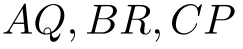
\includegraphics[width=68.36pt]{images-full/p228-i007.png}}\allowbreak{} 交于一点当且仅当三点\allowbreak{}\raisebox{-2.76pt}{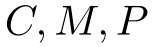
\includegraphics[width=43.50pt]{images-full/p228-i008.png}}\allowbreak{}共线，这又等价于
\sourceblock{296.06}{images-full/p228-d006.png}
也就是\allowbreak{}\raisebox{-2.88pt}{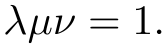
\includegraphics[width=45.35pt]{images-full/p228-i009.png}}\allowbreak{}口
【注4.2.2 】这里，我们看到仿射坐标系在求解几何问题时也具有明显的优越性.
\sourceblock{320.92}{images-full/p228-d007.png}
\par\medskip\noindent\textbf{【例4.3.1 】(第一届全国决赛题)设\allowbreak{}\raisebox{-3.00pt}{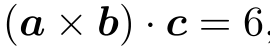
\includegraphics[width=75.77pt]{images-full/p228-i010.png}}\allowbreak{}，则}
\sourceblock{224.87}{images-full/p228-d008.png}


% SOURCE_PDF_PAGE 229

\hypertarget{source-p229}{}
解利用向量运算的性质，得
\sourceblock{337.30}{images-full/p229-d000.png}
【点评】本题相对容易些，主要是测试参赛学生掌握基础知识的熟练程度.
\par\medskip\noindent\textbf{【例4.3.2 】(Putna皿试题)己知\allowbreak{}\raisebox{-2.28pt}{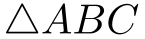
\includegraphics[width=40.68pt]{images-full/p229-i000.png}}\allowbreak{} 的面积为1，点\allowbreak{}\raisebox{-2.76pt}{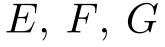
\includegraphics[width=46.33pt]{images-full/p229-i001.png}}\allowbreak{}分别在边\allowbreak{}\raisebox{-2.76pt}{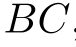
\includegraphics[width=21.39pt]{images-full/p229-i002.png}}\allowbreak{}，}
\allowbreak{}\raisebox{-2.76pt}{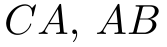
\includegraphics[width=46.89pt]{images-full/p229-i003.png}}\allowbreak{} 上，并且\allowbreak{}\raisebox{-2.40pt}{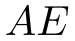
\includegraphics[width=20.90pt]{images-full/p229-i004.png}}\allowbreak{} 于点$R$ 处平分\allowbreak{}\raisebox{-2.64pt}{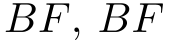
\includegraphics[width=48.02pt]{images-full/p229-i006.png}}\allowbreak{} 于点$S$ 处平分\allowbreak{}\raisebox{-2.76pt}{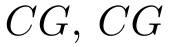
\includegraphics[width=47.40pt]{images-full/p229-i008.png}}\allowbreak{} 于点$T$ 处平分
\allowbreak{}\raisebox{-2.28pt}{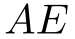
\includegraphics[width=20.85pt]{images-full/p229-i010.png}}\allowbreak{} ( 图4.3.1). 求\allowbreak{}\raisebox{-2.40pt}{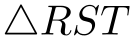
\includegraphics[width=38.42pt]{images-full/p229-i011.png}}\allowbreak{} 的面积.
\sourceblock{105.09}{images-full/p229-d001.png}
圄4.3.1
\sourceblock{249.16}{images-full/p229-d002.png}
\sourceblock{312.44}{images-full/p229-d003.png}
\sourceblock{339.00}{images-full/p229-d004.png}
\sourceblock{383.07}{images-full/p229-d005.png}
另一方面，由(4.3.1) 式与(4.3.2) 式，有
\sourceblock{312.44}{images-full/p229-d006.png}


% SOURCE_PDF_PAGE 230

\hypertarget{source-p230}{}
\phantomsection\addcontentsline{toc}{section}{4.4 能力拓展与训练}
根据对称性，有
\sourceblock{277.98}{images-full/p230-d000.png}
\sourceblock{376.85}{images-full/p230-d001.png}
【点评】对于求平面图形的面积、空间区域的体积等几何问题，用向量方法通常无
需作辅助线，而且往往能降低运算的复杂性.
\sourceblock{320.92}{images-full/p230-d002.png}
\sourceblock{450.00}{images-full/p230-d003.png}
2. 证明:任意四面体的每一个顶点与其对面重心的连线交于一点，且交点与顶点之
间的距离等于它到对面重心距离的3 倍.
3.己知\allowbreak{}\raisebox{-2.40pt}{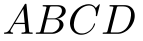
\includegraphics[width=40.11pt]{images-full/p230-i000.png}}\allowbreak{} 是平面内一个凸四边形，\allowbreak{}\raisebox{-2.40pt}{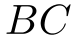
\includegraphics[width=21.47pt]{images-full/p230-i001.png}}\allowbreak{} 平行于\allowbreak{}\raisebox{-2.76pt}{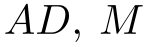
\includegraphics[width=41.81pt]{images-full/p230-i002.png}}\allowbreak{} 是\allowbreak{}\raisebox{-2.40pt}{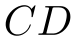
\includegraphics[width=21.47pt]{images-full/p230-i003.png}}\allowbreak{} 的中点，$P$ 是
\sourceblock{450.00}{images-full/p230-d004.png}
\sourceblock{236.73}{images-full/p230-d005.png}
5. 设\allowbreak{}\raisebox{-2.40pt}{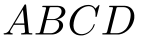
\includegraphics[width=40.11pt]{images-full/p230-i005.png}}\allowbreak{} 是一个对棱长度均相等的四面体，且3 对对棱长度分别为4 ，5, 6，试求
\sourceblock{450.00}{images-full/p230-d006.png}
7.证明:直角三棱锥的斜面(底面)面积的平方等于三个直角面(侧面)面积的平
方和.
8. 在\allowbreak{}\raisebox{-2.28pt}{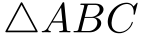
\includegraphics[width=40.68pt]{images-full/p230-i006.png}}\allowbreak{} 中，\allowbreak{}\raisebox{-2.28pt}{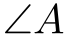
\includegraphics[width=19.77pt]{images-full/p230-i007.png}}\allowbreak{} 不是直角，点\allowbreak{}\raisebox{-2.76pt}{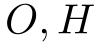
\includegraphics[width=28.25pt]{images-full/p230-i008.png}}\allowbreak{} 分别是\allowbreak{}\raisebox{-2.28pt}{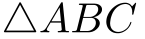
\includegraphics[width=40.68pt]{images-full/p230-i009.png}}\allowbreak{} 的外心与垂心，问: \allowbreak{}\raisebox{-2.28pt}{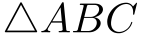
\includegraphics[width=40.68pt]{images-full/p230-i010.png}}\allowbreak{}
满足什么条件时才能使得\allowbreak{}\raisebox{-2.40pt}{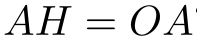
\includegraphics[width=55.52pt]{images-full/p230-i011.png}}\allowbreak{} 请阐述理由


% SOURCE_PDF_PAGE 231

\hypertarget{source-p231}{}
\phantomsection\addcontentsline{toc}{section}{4.5 训练全解与分析}
\sourceblock{450.00}{images-full/p231-d000.png}
以点\allowbreak{}\raisebox{-2.40pt}{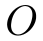
\includegraphics[width=11.86pt]{images-full/p231-i000.png}}\allowbreak{}为球心的一个球面上.
\sourceblock{320.92}{images-full/p231-d001.png}
1.解因为
\sourceblock{241.25}{images-full/p231-d002.png}
\sourceblock{320.92}{images-full/p231-d003.png}
所以\allowbreak{}\raisebox{-3.36pt}{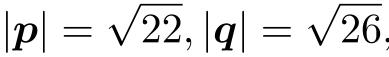
\includegraphics[width=109.81pt]{images-full/p231-i001.png}}\allowbreak{}，从而有
\sourceblock{232.21}{images-full/p231-d004.png}
\sourceblock{272.89}{images-full/p231-d005.png}
2. 证明考虑四面体\allowbreak{}\raisebox{-2.40pt}{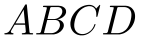
\includegraphics[width=40.11pt]{images-full/p231-i002.png}}\allowbreak{} 的顶点$A$ 与其对面\allowbreak{}\raisebox{-2.74pt}{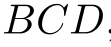
\includegraphics[width=30.93pt]{images-full/p231-i004.png}}\allowbreak{}，设$G$ 是\allowbreak{}\raisebox{-2.40pt}{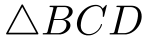
\includegraphics[width=42.37pt]{images-full/p231-i006.png}}\allowbreak{} 的重心，
\sourceblock{450.00}{images-full/p231-d006.png}
\sourceblock{237.30}{images-full/p231-d007.png}
\sourceblock{284.76}{images-full/p231-d008.png}
将(4.5.1) 式代入(4.5.2) 式，得
\sourceblock{180.23}{images-full/p231-d009.png}
同理，对于四面体\allowbreak{}\raisebox{-2.40pt}{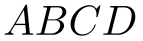
\includegraphics[width=40.11pt]{images-full/p231-i007.png}}\allowbreak{} 的其他三个顶点，在连接顶点与对面重心的线段上作分割
比为3:1 的分点\allowbreak{}\raisebox{-2.40pt}{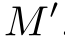
\includegraphics[width=18.01pt]{images-full/p231-i008.png}}\allowbreak{}，也有
\sourceblock{183.62}{images-full/p231-d010.png}


% SOURCE_PDF_PAGE 232

\hypertarget{source-p232}{}
\sourceblock{219.22}{images-full/p232-d000.png}
因此，四面体的顶点与对面重心的连线交于一点，且交点与顶点之间的距离等于它到
\sourceblock{450.00}{images-full/p232-d001.png}
\sourceblock{386.46}{images-full/p232-d002.png}
所以
\sourceblock{250.29}{images-full/p232-d003.png}
\sourceblock{450.00}{images-full/p232-d004.png}
\sourceblock{131.08}{images-full/p232-d005.png}
注意到
\sourceblock{297.19}{images-full/p232-d006.png}
\sourceblock{205.09}{images-full/p232-d007.png}
\sourceblock{377.98}{images-full/p232-d008.png}
所以
\sourceblock{295.49}{images-full/p232-d009.png}


% SOURCE_PDF_PAGE 233

\hypertarget{source-p233}{}
\sourceblock{90.40}{images-full/p233-d000.png}
\sourceblock{450.00}{images-full/p233-d001.png}
\sourceblock{209.05}{images-full/p233-d002.png}
\sourceblock{431.66}{images-full/p233-d003.png}
\sourceblock{340.13}{images-full/p233-d004.png}
由于\allowbreak{}\raisebox{-3.48pt}{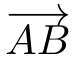
\includegraphics[width=20.90pt]{images-full/p233-i000.png}}\allowbreak{}豆与\allowbreak{}\raisebox{-3.60pt}{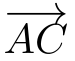
\includegraphics[width=20.90pt]{images-full/p233-i001.png}}\allowbreak{}线性无关所以
\sourceblock{199.44}{images-full/p233-d005.png}
\sourceblock{450.00}{images-full/p233-d006.png}
对空间任意一点\allowbreak{}\raisebox{-2.76pt}{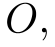
\includegraphics[width=15.25pt]{images-full/p233-i002.png}}\allowbreak{}，有
\sourceblock{371.77}{images-full/p233-d007.png}


% SOURCE_PDF_PAGE 234

\hypertarget{source-p234}{}
\sourceblock{450.00}{images-full/p234-d000.png}
\sourceblock{347.47}{images-full/p234-d001.png}
\sourceblock{132.21}{images-full/p234-d002.png}
所求四面体的体积为
\sourceblock{270.07}{images-full/p234-d003.png}
\sourceblock{391.54}{images-full/p234-d004.png}
将以上三式一并代入上述Gram 矩阵，得到行列式
\sourceblock{242.38}{images-full/p234-d005.png}


% SOURCE_PDF_PAGE 235

\hypertarget{source-p235}{}
因此，所求四面体的体积为
\sourceblock{267.81}{images-full/p235-d000.png}
\sourceblock{433.92}{images-full/p235-d001.png}
的法向量.显然，若记\allowbreak{}\raisebox{-1.68pt}{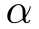
\includegraphics[width=10.73pt]{images-full/p235-i000.png}}\allowbreak{}为平面\allowbreak{}\raisebox{-2.40pt}{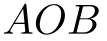
\includegraphics[width=29.94pt]{images-full/p235-i001.png}}\allowbreak{} 与平面\allowbreak{}\raisebox{-2.40pt}{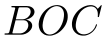
\includegraphics[width=30.51pt]{images-full/p235-i002.png}}\allowbreak{} 的二面角，则\allowbreak{}\raisebox{-3.00pt}{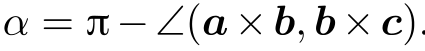
\includegraphics[width=119.60pt]{images-full/p235-i003.png}}\allowbreak{}.
\sourceblock{328.83}{images-full/p235-d002.png}
利用Lagrange 恒等式:对任意\allowbreak{}\raisebox{-2.16pt}{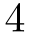
\includegraphics[width=9.04pt]{images-full/p235-i004.png}}\allowbreak{}个向量\allowbreak{}\raisebox{-3.24pt}{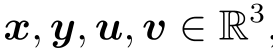
\includegraphics[width=77.05pt]{images-full/p235-i005.png}}\allowbreak{}，有
\sourceblock{393.24}{images-full/p235-d003.png}
\sourceblock{450.00}{images-full/p235-d004.png}
\sourceblock{396.06}{images-full/p235-d005.png}
\sourceblock{401.71}{images-full/p235-d006.png}


% SOURCE_PDF_PAGE 236

\hypertarget{source-p236}{}
\sourceblock{450.00}{images-full/p236-d000.png}
\sourceblock{237.86}{images-full/p236-d001.png}
\sourceblock{450.00}{images-full/p236-d002.png}
\sourceblock{118.08}{images-full/p236-d003.png}
\sourceblock{327.70}{images-full/p236-d004.png}
【注4.5.1 】这里，需要熟悉平面几何中的一个己知结论，即Euler 线定理:三角形
的外心、重心和垂心共线，且外心和重心的距离是垂心和重心的距离一半(图4.5.3).
\sourceblock{120.34}{images-full/p236-d005.png}
\sourceblock{326.00}{images-full/p236-d006.png}
\sourceblock{339.56}{images-full/p236-d007.png}
于是，有
\sourceblock{357.08}{images-full/p236-d008.png}


% SOURCE_PDF_PAGE 237

\hypertarget{source-p237}{}
由于
\sourceblock{379.11}{images-full/p237-d000.png}
\sourceblock{408.49}{images-full/p237-d001.png}
\sourceblock{67.80}{images-full/p237-d002.png}
